\subsection{Methods} 

\subsubsection{Network pipeline}

% Start by giving an overview of the pipeline, there are several components to it: Network contruction & gene filtering, Community Detection, Finding the relevant genes in each community, Representation of this genes across samples & clustering
From Figure \ref{fig:N_I:network_pipeline} The network pipeline is broken in several stages 1) the network is constructed based on the filtered genes 2) detecting  communities 3) find the most important genes in each community and 4) Find the representation of the genes from 3) to the samples and then apply clustering analysis. 

% Describe each componenet and why I'm doing this 

%% Gene filtering will be with Network Construction
The genes are filtered by the same approach as in \ref{} selecting the top 5K genes (depending on the experiment) that have the highest median/standard deviation. A Spearman Correlation matrix is then built on the 5K genes, where the correlation between two genes represents the edges' weight while the genes are the network nodes. For a network of 5K nodes there are $1.24x10^6$ combinations, making it very difficult to analyse. Thus, a selective edge pruning strategy needs to used.

% Selective edge pruning

% Community detection

% Finding the relevant genes

% Representation of genes across samples & Clustering

\newline
Things to cover in the pipeline:
\begin{todolist}
    \item Gene selection
    \item Combination of multiple datasets
    \item Edges per node
    \item Correlation
    \item Community detection
    \item Module Community scores
    \item Module Evaluation Value
    \item Hierarchical clustering
    \item Visualising with Gephi
\end{todolist}

\subsubsection{Modified PGCNA}

Clearly separate the modifications I made to PGCNA and explain the reason behind them:

\begin{itemize}
    \item Already implemented:
          \begin{itemize}
              \item Allow more edges per node for the Transcription Factors (TF)
              \item Modify the pipeline to export the graph objects outside of the PGCNA developed by Mathew Care
              \item Add the modifiers to the genes to penalise/reward based on the mutation count.
              \item Change the community detection algorithm from Leiden to stochastic block model (SBM)(Zhang and Peixoto 2020). I read some criticism (blog, paper) of the current approaches in community detection and I want to explore the suggested alternative SBM.
          \end{itemize}
    \item On the list
    \begin{itemize}
        \item More integrative MEV approach
    \end{itemize}
\end{itemize}

\subsubsection{Figures} 


\begin{figure}[!htb]
    \centering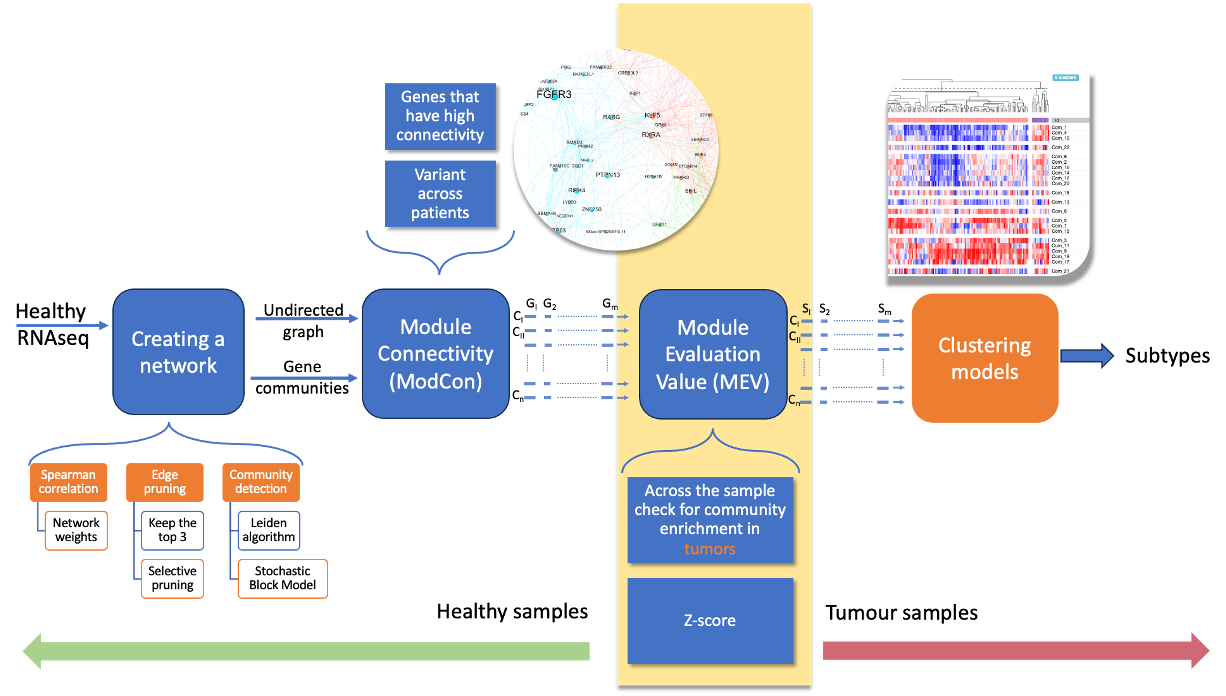
\includegraphics[width=0.75\textwidth,height=0.75\textheight,keepaspectratio]{Sections/Network_I/Resources/Methods/network_pipeline.png}
    \caption{Network pipene}
    \label{fig:N_I:network_pipeline}
\end{figure}



% \subsubsection{Building a network}

% \subsubsection{Analysing a network}

% \subsubsection{Finding communities}

% \subsubsection{Integrating data}

% \subsubsection{From gene communities back to samples subtypes}

% \subsubsection{Biological interpretation}